\documentclass[12pt, oneside, reqno]{article}
\usepackage{amssymb, amsthm, amsmath, amsfonts}
\usepackage{fancybox}
\usepackage{graphicx}
\usepackage{amsrefs}
\usepackage{color}
\usepackage{bardtex}
\usepackage{verbatim}
\usepackage{fancyhdr}

\styleoption{prospectus}

\usepackage{fourier}

%The following four optional commands change the colors in the poster; if you want to change the default colors, use any or all of these four commands by removing the % symbols, and inserting your choice of colors.  See the manual for details about colors in posters.
%\prospectustitlecolor{color}
%\prospectusnamecolor{color}
%\prospectusheadingtextcolor{color}
%\prospectusheadingbackgroundcolor{color}


%Your macros, if you have any.


\begin{document}

\titleprospectus{Why I Love Mathematics}{Angela Albee}{Mathematics Program}{October 2099}{Calvin Calculus}


\startmain

\prospectusslideone{About the Prospectus Template}

The prospectus template, which is part of the \textsf{bardtex.sty} style file, is an easy-to-use, though not very fancy, template for mathematics talks.

This template has the following features.

\begin{itemizecp}{Magenta}
\item 
The template has a title slide, slides for content and references slides.

\item
The template produces only very basic slides, which are completely static, and have no dynamic features such as bullet points that appear one at a time.

\item
Because this template is part of the ``bardtex suite,'' the same commands for theorems, proofs, and the like that are used for other templates associated with the style file, for example the template for senior projects, can also be used here.

\item
As you have likely noticed, there is a built-in method for itemized lists with colored bullets, with your choice of colors. 
\end{itemizecp}


\prospectusslidetwo{More Things about the Prospectus Template}

\begin{enumeratecp}{Cyan}
\item 
There is also a built-in method for enumerated lists with colored numbers, with your choice of colors.

\item
Every page has a title, which is highlighted with a colored strip.

\item
In this template there are four built-in colors, all of which have default values, but which can be changed with commands that are available in the preamble to the .tex file.  The built-in colors are the color of the title of the project, the color of the name of the student, the color of the text in the heading strip at the top of each slide, and the color of the heading strips.

\item
The default font for this template is \verb@fourier@, though oher TeX fonts can be used too.  Strangely, Computer Modern fonts (the default TeX font), in addition to not looking very nice (according to some opinions), does not work properly with the title page of this template, and so should not be used.

\item
Prospectus talks should be at most five slides, and each slide should be one page, no more!  If you accidentally write the text of a slide and it goes over one page---as is the case with this remark---you will notice it because the page with the overflow will not have a heading.  Please stick to five slides or fewer, where each slide is a single page.

\end{enumeratecp}


\prospectusslidethree{Various Things}

The text in each slide is typed using standard LaTeX, as in the displayed formula
%
\[
\prod_{i \in I} A_i = \{f \in \funcspce I{\bigcup_{i \in I} A_i} \mid f(i) \in A_i \text{ for all } i \in I\}. 
\]
%

Figures should be inserted as for the poster template associated with the \textsf{bardtex.sty} style file, that is, without 
\begin{center}
\verb@\begin{figure} ... \end{figure}@. 
\end{center}
The method of inserting figures is explained in the manual for the style file.

\begin{center}
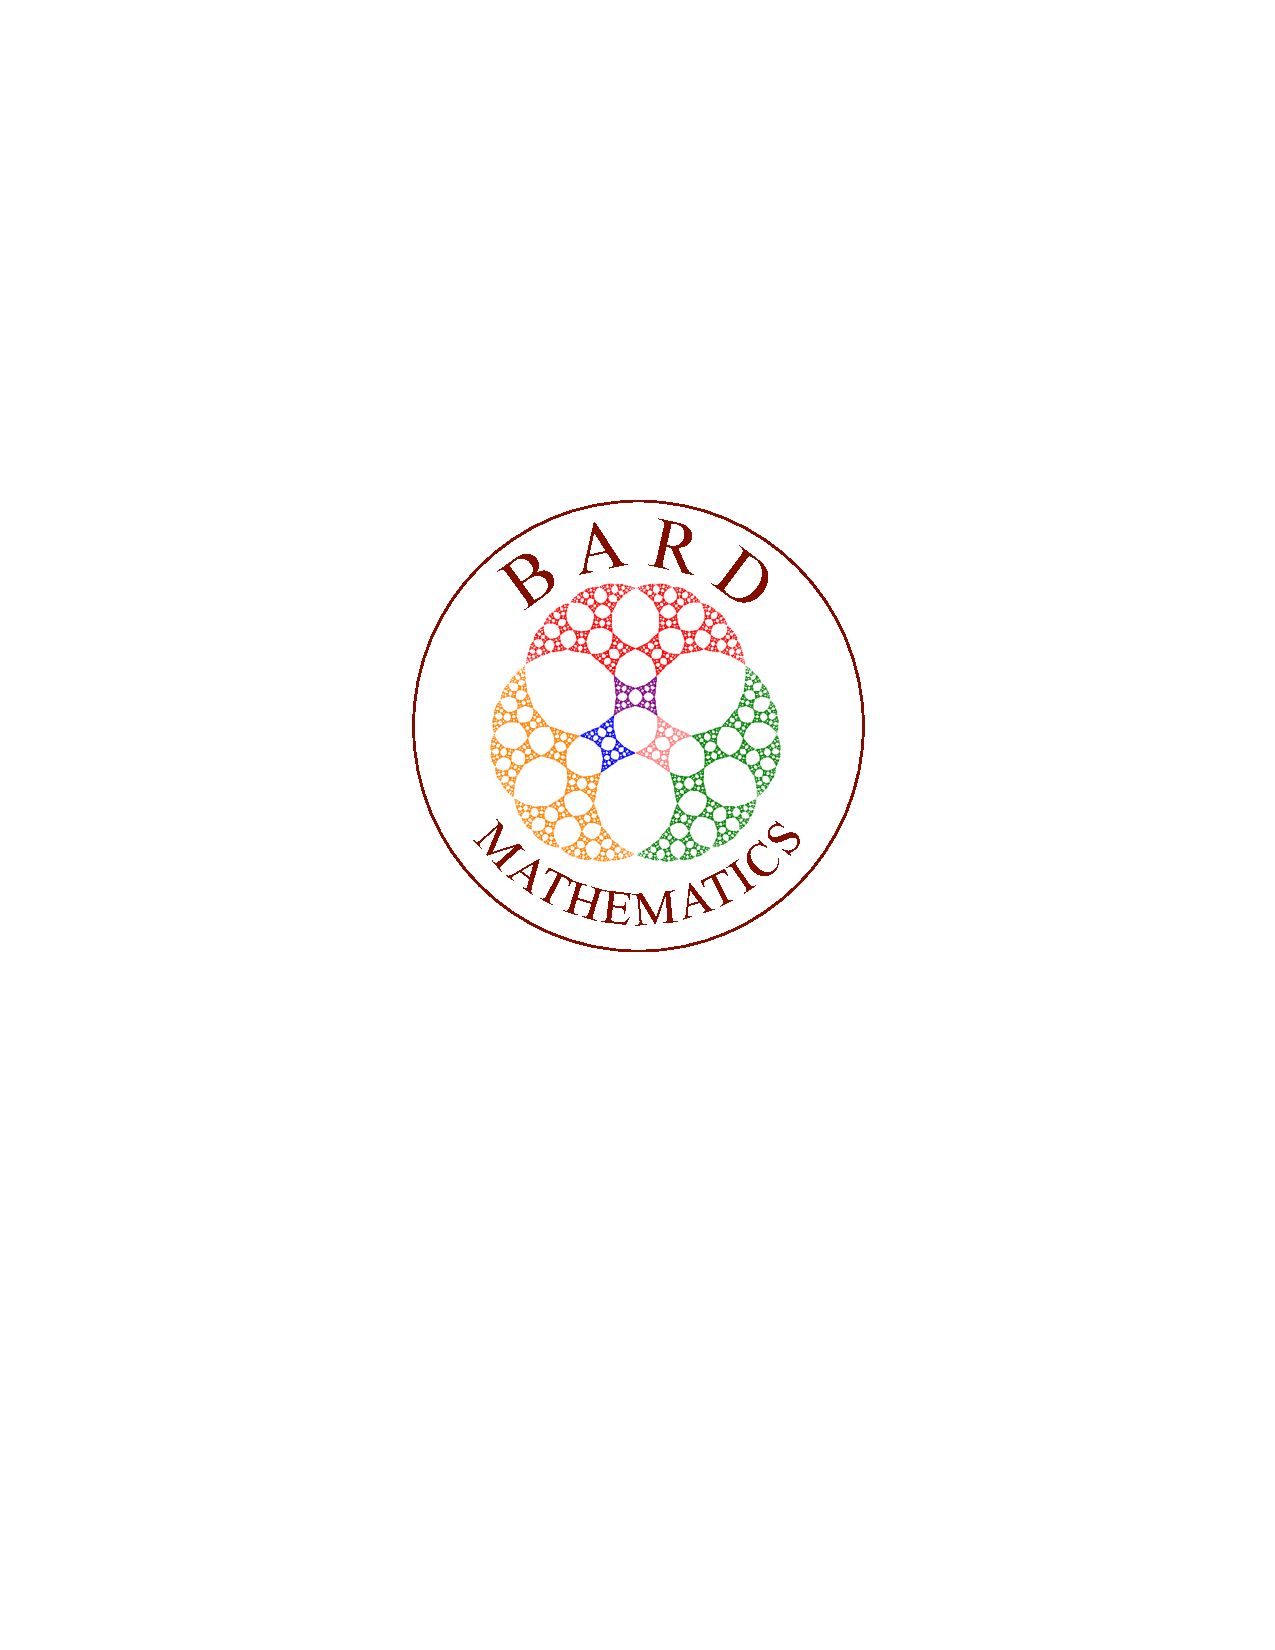
\includegraphics[scale=0.75]{math_prog_logo.pdf}\\
Figure 1: The Bard Mathematics Program Logo
\end{center}


\prospectusslidefour{More Various Things}

On the following page is a theorem and proof taken from the Proofs and Fundamentals book.

On the page after that, there is a short bibliography.  The bibliography was copied verbatim from the poster sample file (except that the title of the third item was changed).  The style file adjusts the appearance of the bibliography depending upon the choice of template.

It looks nicer in slides when enumerated and itemized lists are used, rather than having text in normal paragraphs, but, as seen on this page, normal paragraphs can be used too if someone so chooses.

Slides do not have to be filled.

\prospectusslidefive{A Theorem and Proof}

\thm\label{thmAA} 
Let $\func fAB$ be a function.
%
\enum 
\item[(1)] If $f$ has an inverse, then the inverse is unique.
%
\item[(2)] If $f$ has a right inverse $g$ and a left inverse $h$, then $g = h$; hence $f$ has an inverse.
%
\item[(3)] If $f$ has an inverse $g$, then $g$ has an inverse, which is $f$.
\eenum
\ethm
 
\demo
(1). Suppose that $\func {g, h}BA$ are both inverses of $f$.  We will show that $g = h$.  By hypothesis on $g$ and $h$ we know, among other things, that $f \circ g = 1_B$ and $h \circ f = 1_A$.  Using a previous lemma we see that
%
\[
g  =  1_A \circ g  =  (h \circ f) \circ g  =  h \circ (f \circ g)  =  h \circ 1_B  =  h.
\]

\noindent (2). The proof is virtually the same as in Part~(1).  
\spce

\noindent (3).  Since $\func gBA$ is an inverse of $f$, then $g \circ f = 1_A$ and $f \circ g = 1_B$.  By the definition of inverses, it follows that $f$ is an inverse of $g$.  By Part~(1) of this theorem, we know that $f$ is the unique inverse of $g$.
\edemo

\begin{bibliog}

\bib{HOMOLOGY}{book}{
author = {Homology, Harold},
title = {Algebraic Topology for Dummies},
publisher = {Math Lights},
address = {Simplicialville, NY},
date = {2099}
}

\bib{CALCULUS}{article}{
author = {Calculus, Cathy},
title = {Why everyone should love calculus},
journal = {Journal of Fun Mathematics},
volume = {314},
date = {2099},
pages = {100--101}
}

\bib{POSTER}{report}{
author = {Function, Felicity},
author = {Tangent, Tim},
title = {How to Give a Great Mathematics Talk},
eprint = {http://www.www.www.edu}
}

\end{bibliog}

\end{document}

